\chapter[Algorithme de propagation d'interfaces régulières par~morceaux]{Algorithme général pour la propagation d'interfaces régulières par~morceaux}
\label{chap:algo_general}


L'objet de ce chapitre est de mettre au point un algorithme général basé sur le principe de Huygens (avec condition d'entropie) pour simuler la propagation d'une interface géométriquement régulière par morceaux. 
On représente l'interface sous la forme d'un modèle \brep. L'algorithme vise alors à construire un nouveau modèle \brep\ (géométrie et topologie) correspondant à une enveloppe de boules (EdB) centrées sur l'interface courante. 


%\textit{on veut mettre en place un algorithme basé sur le principe de Huygens (avec condition d'entropie) pour simuler la propagation d'une interface représentée suivant le formalisme \brep, i.e. pour construire un nouveau modèle \brep\ (géométrie et topologie) correspondant à une enveloppe de boules (EdB) centrées sur l'interface courante.}


\section{Traitement des différentes entités \brep}
on construit d'abord une EdS (partielle), puis on la transforme en EdB pour respecter la condition d'entropie. Chaque entité du modèle \brep\ est traitée spécifiquement

vitesse normale continue $\Rightarrow$ rayon des sphères évolue continument 
sur toute l'interface
\subsection{Traitement des faces}
chaque face repose sur une surface orientée de continuité géométrique élevée (d'ordre 1 ou plus) donc chaque point sur une face a exactement 2 vis-à-vis sur l'EdS (un dans le sens de la normale, et un dans le sens opposé) (sous réserve d'une condition, détaillée dans la \autoref{sec:EdS_2param})


\subsection{Traitement des arêtes}
\begin{itemize}
	\item douce $\to$ préservée car vitesse continue ;
	\item (vive) convexe $\to$ EdS à un paramètre (nouvelle \textit{sur}face) ;
	\item (vive) concave $\to$ aucune influence sur l'EdB (on ne construit pas son EdS, d'où le ``partiel'') ;
\end{itemize}

\subsection{Traitement des sommets}
\begin{itemize}
	\item smooth $\to$ préservé car vitesse continue ;
	\item convexe $\to$ nouvelle(s) \textit{sur}face(s) sphérique(s) ;
	\item concave $\to$ aucune influence sur l'EdB.
\end{itemize}


%\begin{itemize}
%	\item faces $\to$ EdS à deux paramètres (justifier) ;
%	\item arêtes
%	\begin{itemize}
%		\item douce $\to$ préservée car vitesse continue ;
%		\item (vive) convexe $\to$ EdS à un paramètre (nouvelle(s) \textit{sur}face(s)) ;
%		\item (vive) concave $\to$ aucune influence sur l'EdB (on ne construit pas son EdS, d'où le ``partiel'') ;
%	\end{itemize}
%	\item sommets
%	\begin{itemize}
%		\item smooth $\to$ préservé car vitesse continue ;
%		\item convexe $\to$ nouvelle(s) \textit{sur}face(s) sphérique(s) ;
%		\item concave $\to$ aucune influence sur l'EdB.
%	\end{itemize}
%\end{itemize}

%\section{Ce titre de section est vraiment trop long,\newline il faudrait trouver un moyen de le raccourcir,\newline il s'étend sur plusieurs lignes, c'est beaucoup trop long}


\section{Construction de l'enveloppe des sphères}%{Construction géométrique de l'enveloppe des sphères}

\subsection{Enveloppe d'une famille de sphères à un paramètre}
%\subsection{Enveloppe d'un ensemble de sphères à un paramètre}
\eng{canal surfaces} \cite{peternell1997} (\eng{spine curve} $\to$ squelette (ou axe médian))

\begin{figure}[!htp]
	\centering
	\begin{tikzpicture}[
		scale=1.4,
		point/.style = {circle, scale=0.27, fill=black},
		vector/.style = {-latex', thick},
		label/.style = {inner sep=1pt},
		txt/.style = {font=\small}]
		\node[anchor=north west, inner sep=0] at (0,0) {\includegraphics[width=112mm]%width=scale*80mm
		{figures/canal_surface4}};
		\coordinate (g) at (27.4114285714mm,-31.2685714286mm);
		\node [point] at (g) {};
		%\node [anchor=north east, label, txt] at (g) {$\bg(u)$};
		\node [anchor=south west, label, txt] at (g) {$\bg$};
		\coordinate (p) at (19.8628571429mm,-21.68mm);
		\node [anchor=west, txt] at (p) {$\boldsymbol{\phi}(u,v)$};
		\node [point] at (p) {};
		\coordinate (q) at ($(g)!1.8!(p)$);
		\node [anchor=south west, label, txt, xshift=-5pt]
		at (q) {$\mathbf{q}(u,v)$};
		\draw [dotted, thick] (g) -- (p);
		\draw [vector] (p) -- (q);
		\coordinate (dgmax) at (80mm,-37.8114285714mm);
		\coordinate (dg) at ($(g)!0.5!(dgmax)$);
		\draw [vector] (g) -- (dg) node [above right, label, txt, xshift=-2pt] {$\bg_u(u)$};
		\draw [stealth-stealth, shorten <= 2.2pt, shorten >= 1.5pt] (g) -- node[pos=0.45, right, txt] {$\rho(u)$} (36.1771428571mm,-43.7257142857mm);
		\node [txt, label, anchor=south east] at (71.0857142857mm,-19.2mm) {$\Gamma$};
		\definecolor{charcirc_clr}{HTML}{105DFF}
		\node [txt, label, anchor=south west, charcirc_clr] at 
		(18.3714285714mm,-41.2mm) %(17.7428571429mm,-38.5142857143mm) 
		{$\mathscr{C}(u)$};
		\node [txt, label, anchor=south, charcirc_clr] at 
		(31.3142857143mm,-8.6mm)%(16.2857142857mm,-53.7142857143mm) 
		{$\mathscr{P}(u)$};
		\definecolor{envelope_clr}{HTML}{40C516}
		\node [txt, label, anchor=south east, envelope_clr] at (47.6571428571mm,-3.7714285714mm) {$\Phi$};
		\definecolor{sphere_clr}{rgb}{0.799,0.396,0.159}
		\node [txt, label, sphere_clr] at (36.7mm,-23.8mm) {$\mathscr{S}(u)$};
		\coordinate (o) at (23.8893473148mm,-30.8355408822mm);
		\draw [dashed] (o) -- (g);
		\node [point] at (o) {};
		\node [txt, label, below left] at (o) {$\vrm{o}$};
		\draw [stealth-stealth, shorten <= 2.2pt, shorten >= 2.2pt] (o) -- node[pos=0.5, left, txt] {$r$} (p);
	\end{tikzpicture}
\end{figure}

%\begin{figure}[!htp]
%	\centering
%	\begin{tikzpicture}[
%		scale=1.5,
%		point/.style = {circle, scale=0.27, fill=black},
%		vector/.style = {-latex', thick},
%		label/.style = {inner sep=1pt},
%		txt/.style = {font=\small}]
%		\node[anchor=north west, inner sep=0] at (0,0) {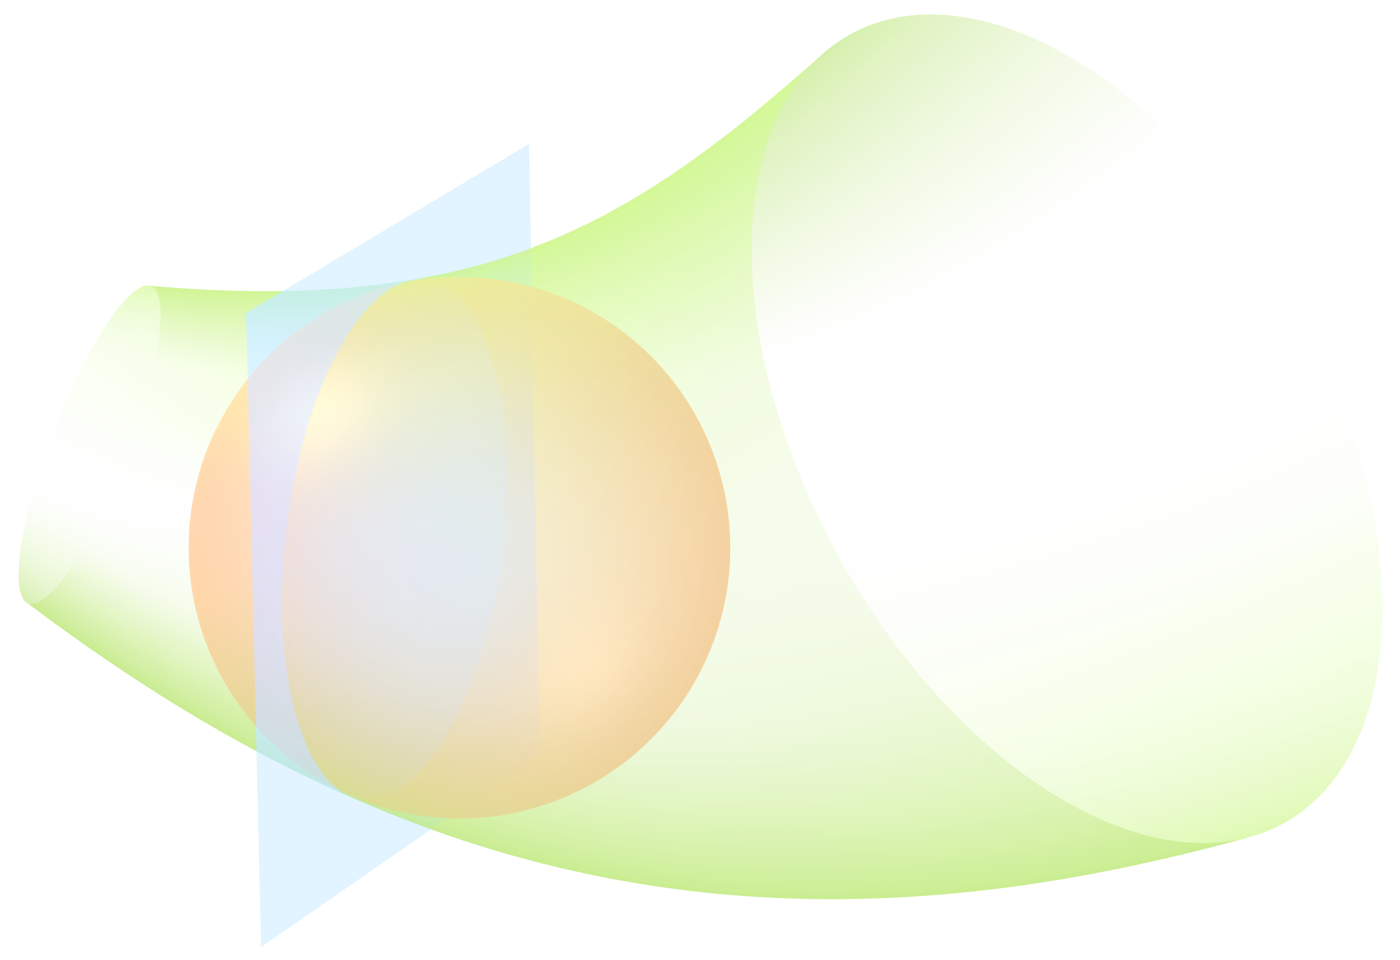
\includegraphics[width=12cm]{figures/canal_surface2_spec}};
%		\coordinate (g) at (29.704mm,-31.32mm);
%		\node [point] at (g) {};
%		\node [anchor=north east, label, txt] at (g) {$\bg(u)$};
%		\coordinate (p) at (22.752mm,-22.512mm);
%		\node [anchor=west, txt] at (p) {$\boldsymbol{\phi}(u,v)$};
%		\node [point] at (p) {};
%		\coordinate (q) at ($(g)!1.8!(p)$);
%		\node [anchor=south west, label, txt, xshift=-5pt]
%		at (q) {$\mathbf{q}(u,v)$};
%		\draw [dotted, thick] (g) -- (p);
%		\draw [vector] (p) -- (q);
%		\coordinate (dgmax) at (80.0mm,-37.56mm);
%		\coordinate (dg) at ($(g)!0.5!(dgmax)$);
%		\draw [vector] (g) -- (dg) node [above right, label, txt, xshift=-2pt] {$\bg_u(u)$};
%		\draw [thick, stealth-stealth, shorten <= 2.2pt, shorten >= 1.5pt] (g) -- node[pos=0.4, right, txt] {$r(u)$} (37.52mm,-43.0mm);
%	\end{tikzpicture}
%\end{figure}


\subsection{Enveloppe d'une famille de sphères à deux paramètres}
\label{sec:EdS_2param}
extension \eng{canal surfaces} \cite{gelston1995}\\
différence avec le simple transport suivant la normale \cite{jiao2001}


\begin{figure}[!htp]
	\centering
	\begin{tikzpicture}[
		scale=1.5,
		point/.style = {circle, scale=0.27, fill=black},
		vector/.style = {-latex', thick},
		label/.style = {inner sep=2pt},
		txt/.style = {font=\small}]
		\node[anchor=north west, inner sep=0] at (0,0) {\includegraphics[width=12cm]%width=scale*80mm
		{figures/2pEoS_nointer}};
		\coordinate (s) at (40.632mm,-21.936mm);
		%
		\coordinate (pp) at (38.4mm,-9.56mm);
		%\node [anchor=west, txt] at (pp) {$\eos_+$};
		\node [anchor=north, txt, xshift=3pt, label] at (pp) {$\eos_+$};
		\coordinate (pm) at (38.76mm,-32.4mm);
		%\node [anchor=west, txt] at (pm) {$\eos_-$};
		\node [anchor=south, txt, xshift=3pt, label] at (pm) {$\eos_-$};
		%
		\coordinate (svmax) at (8.416mm,-34.856mm);
		\coordinate (sv) at ($(s)!-0.55!(svmax)$);
		\draw [vector, blue] (s) -- (sv) node [above, label, txt] {$\bs_v$};
		\coordinate (sumax) at (60.872mm,-35.28mm);
		\coordinate (su) at ($(s)!0.65!(sumax)$);
		\draw [vector, red] (s) -- (su) node [right, label, txt] {$\bs_u$};
		%
		\coordinate (nmax) at (40.472mm,-6.176mm);
		\coordinate (n) at ($(s)!0.4!(nmax)$);
		\draw [vector] (s) -- (n) node [right, label, txt, black] {$\unv$};
		%
		\coordinate (qp) at ($(s)!1.6!(pp)$);
		\node [anchor=west, label, txt, xshift=0pt]
		at (qp) {$\mathbf{q}_+$};
		\draw [dotted, thick, shorten >= 14pt] (s) -- (pp);
		\draw [vector] (pp) -- (qp);
		%
		\coordinate (qm) at ($(s)!1.6!(pm)$);
		\node [anchor=east, label, txt, xshift=0pt]
		at (qm) {$\mathbf{q}_-$};
		\draw [dotted, thick, shorten <= 0pt, shorten >= 14pt] (s) -- (pm);
		\draw [vector] (pm) -- (qm);
		%
		\node [point] at (s) {};
		\node [point] at (pp) {};
		\node [point] at (pm) {};
		%
%		\node [anchor=north, txt, inner sep=3pt] at (s) {$\bs(u,\!v)$};
		%\node [anchor=west, txt, inner sep=4pt] at (s) {$\bs(u,\!v)$};
		\node [anchor=east, txt, inner sep=2pt] at (s) {$\bs(u,v)$};
		\node [txt, label] at (5.49mm,-15mm) {$\Sigma$};
	\end{tikzpicture}
\end{figure}



\section{Application de la condition d'entropie}
résolution des intersections (pas encore de détail sur la méthode) $\to$ faces trimmées, nouveaux sommets/arêtes

\subsection{Reconstitution topologique du modèle \brep}
Intersections de paires de surfaces ($\to$ courbes\footnote{dans le cas général, non-dégénéré (cf. cours ``Topologie et géométrie différentielle'')\label{foot}}), de triplets de surface (ou de paires de courbes) ($\to$ points\textsuperscript{~\ref{foot}})\\
graphe d'adjacence des surfaces, courbes, points \cite[Chap. 4]{pentcheva2010}\\
formation des faces (\eng{wires} $\to$ chaînes?) \cite[Chap. 7]{pentcheva2010}, arêtes et sommets \cite[Chap. 5]{pentcheva2010}

\ldots
%\convertto{mm}{\textwidth}

%\def\numim{2}%{}
%\def\imw{80mm}
%\def\imh{\imw}
%\def\alp{0.2}
%\def\heoffset{0.013}
%\DTLsetseparator{ }%
%\DTLloaddb[noheader,keys={x,y,a}]{vertdata}{figures/data/demo_EoS_brep_verts.dat}%
%\DTLloaddb[noheader,keys={xa,ya,xb,yb,r,g,b}]{hedgdata}{figures/data/demo_EoS_brep_hedg.dat}%
%\begin{figure}%
%	\centering%
%	\begin{tikzpicture}[
%		x=\imw, y=\imh,
%		img/.style={anchor=south west, inner sep=0},
%		halfedge/.style={thick, -{Triangle[left]}}]
%		%\begin{scope}
%		%	\clip (0.11,0) rectangle (0.928,1);
%			\node [img] at (0,0) {\includegraphics[width=\imw]{figures/demo_brep\numim}};%
%			\node [img] at (0,0) {\includegraphics[width=\imw]{figures/demo_brep_edges_visible\numim}};%
%			{\transparent{\alp}\node [img] at (0,0) {\includegraphics[width=\imw]{figures/demo_brep_edges_hidden\numim}};}%
%			\DTLforeach*{vertdata}{\x=x, \y=y, \a=a}%
%			{%
%				\pgfmathsetmacro\alpi{1 + (1 - \a)*(\alp - 1)}%
%				{\transparent{\alpi}\fill[black] (\x,\y) circle (1pt);}%
%			}%
%			%
%			\DTLforeach*{hedgdata}{\xa=xa,\ya=ya, \xb=xb,\yb=yb, \r=r, \g=g, \b=b}%
%			{%
%				\definecolor{tmpcolor}{rgb}{\r,\g\b}%
%				\draw[tmpcolor, halfedge] (\xa,\ya) -- (\xb,\yb);
%			}%
%%			\draw[blue, halfedge, line cap=round] 
%%			(0.199, {0.2506+0.02}) to[out=340, in=340]
%%			(0.1689, {0.525-0.02});
%		%\end{scope}
%	\end{tikzpicture}%
%\end{figure}%
%\DTLgdeletedb{vertdata}
%
%\def\alp{0}
%\DTLloaddb[noheader,keys={x,y,a}]{vertdata_eos}{figures/data/demo_EoS_brep_verts_new.dat}%
%\begin{figure}
%	\centering
%	\begin{tikzpicture}[
%		x=\imw, y=\imh,
%		img/.style={anchor=south west, inner sep=0}]
%		\node [img] at (0,0) {\includegraphics[width=\imw]{figures/demo_EoS_brep\numim}};%
%		\node [img] at (0,0) {\includegraphics[width=\imw]{figures/demo_EoS_brep_edges_visible\numim}};%
%		{\transparent{\alp}\node [img] at (0,0) {\includegraphics[width=\imw]{figures/demo_EoS_brep_edges_hidden\numim}};}%
%		\DTLforeach*{vertdata_eos}{\x=x, \y=y, \a=a}%
%		{%
%			\pgfmathsetmacro\alpi{1 + (1 - \a)*(\alp - 1)}%
%			{\transparent{\alpi}\fill[black] (\x,\y) circle (1pt);}%
%		}%
%	\end{tikzpicture}
%\end{figure}
%\DTLgdeletedb{vertdata_eos}


\bigskip
\textit{il faut maintenant faire le choix d'une méthode numérique pour appliquer cet algorithme de façon pratique\ldots}